% **************************************************
%   Wichtig für die verwendung der hsrmreport-Klasse!
%
%   Die Datei hsrmreport.cls muss in dem selben Ordner sein
%   wie die .tex Datei die diese Klasse verwenden möchte.
%
%   Desweiteren ist die Dokumentenklasse nach aktuellem
%   noch ohnen Optionen, sprich Zweiseitig, änderung
%   der Schriftgröße oder ähnliches. Ich werde versuchen
%   diese Features hinzu zufügen sobald es mir möglich ist.
%
%   Falls Ihr Probleme, Anregungen oder Verbesserungen habt,
%   könnt ihr mir das gerne mitteilenen.
%
%   Es kann sein das ihr evtl. manche Packete noch installieren
%   müsst bevor die Klasse Fehlerfrei funktioniert.
%   Meldungen wie "Command terminated with space." können ignoriert werden.
%
%   Ich werde auch eine Übersicht aller Pakete schreiben, die ich verwendet habe.
%
%
%   E-Mail: timjonas.wechler@student.hs-rm.de
% **************************************************


\documentclass[printbib, ngerman]{hsrmreport}
% **************************************************
% Ihr könnte die Angaben der TITELSEITE hier ändern
% **************************************************
\newcommand{\titel}{Resistives Touch-Panel}
\newcommand{\studiengang}{Angewandte Physik}
\newcommand{\studienrichtung}{Physikalische Technik}
\newcommand{\dokumentenart}{Laborbericht}
\newcommand{\kurs}{LV:\ Embeeded System Labor}
\newcommand{\versuchsdurchfuehrungDatum}{4. Februrar 2022}
\newcommand{\AbgabeOrt}{Rüsselsheim am Main}

%Falls ihr weniger als vier Studenten seit könnt ihr dies Einträge die zu viel sind einfach löschen.
%Ein Feature für das angeben der Mat.Nr. ist noch in Arbeit.
\newcommand{\studentA}{Dennis Hunter}
\newcommand{\matStudentA}{()}
\newcommand{\studentB}{Tim-Jonas Wechler}
\newcommand{\matStudentB}{(1137877)}
\newcommand{\studentC}{}
\newcommand{\matStudentC}{}
\newcommand{\studentD}{}
\newcommand{\matStudentD}{}

\newcommand{\Referent}{}
\newcommand{\Korreferent}{}


\usepackage{datatool}
\usepackage{babel}
\usepackage{cleveref}
\usepackage{microtype}
\usepackage{listings}
\bibliography{bib-refs_DH}


% Mit dem Befehl \today wird immer das aktuelle Datum auf der Titelseite ausgebeben.
% Wenn dies nicht erwünscht ist einfach manuell das gewünschte Datum eintragen.
\newcommand{\datum}{\today}



\begin{document}
    % **************************************************
    %
    % HIER BEGINNT DER BERICHT
    %
    % **************************************************

    \chapter{Einleitung}
Seit einigen Jahren findet man immer häufiger Bedienungen mit Touchscreens. Ihr Einsatzbereich scheint keine Grenzen zu haben und so hat sich die Technologie in den letzten Jahren rasant weiterentwickelt.


\section{Ziel des Projekts}
In dieser Projektarbeit ist es Ziel, die Aufnahme und Auswertung der Koordinaten mittels eines resistiven Touchscreens. Zum Schluss soll die Steuerung noch dahingehend erweitert werden, dass damit die Maus eines PC's gesteuert werden kann.


\section{Grundlagen}
\subsection{Resistives Touchscreen}
Es gibt bei den resistiven Touchscreens zwei unterschiedliche Gruppen. Zum einen gibt es 4-Wire resistive Touchscreens. Diese haben vier Anschlüsse, über die die Positionsauswertung läuft. 
Zudem gibt es noch die 5-Wire resistive Touchscreens. Hier werden fünf Anschlüsse benötigt um eine Positionsauswertung durchführen zu können. 

Bei einem 4-Wire resistiven Touchscreen gibt es zwei Ebenen, bei denen die obere auf die untere gedrückt werden kann. 
Eine Ebene ist mit Elektronen geladen und über die andere Ebene misst man die Spannung, die bei der Berührung abfällt. 
Für die Andere Richtung ist es das gespiegelt. Die Ebene, die  die Spannung in die eine Richtung misst, ist für die andere Richtung mit Elektronen geladen. Die Messung der Spannung wird dann von der anderen Ebene durchgeführt.
Über die unterschiedliche Beträge der Spannung lässt sich dann die Koordinate in x-Richtung und y-Richtung bestimmen. 

Die 5-Wire resistive Touchscreens haben ebenfalls zwei Ebene. Der Unterschied zu den 4-Wire Touchscreen liegt darin, dass es nur eine Ebene gibt, die geladen ist. Normalerweise ist es die untere Schicht. Die obere Schicht misst für x-Richtung und y-Richtung die abfallende Spannung.
Auch hier wird durch Druck auf die obere Schicht ein Kontakt zwischen den beiden Ebenen erstellt, damit die Messung durchgeführt werden kann. 

Die 5-Wire Touchscreens sind gegenüber den 4-Wire Widerstandsfähiger und haben dadurch eine längere Lebenserwartung.\cite{5w4w}

In diesem Projekt wird ein 4-Wire resistiver Touchscreen von der Firma Fujitsu verwendet.

Der verwendete Touchscreen besitzt für jede Richtung (x und y) jeweils zwei Anschlüsse \figref{fig:4w}. In x, wie auch in y-Richtung sind jeweils 2 Widerstände eingezeichnet. 
Diese sollen den Widerstand auf der jeweiligen Ebene, über die die Spannung abfällt, darstellen.
Die Aufnahme der Werte für einen Koordinatenwert wird über das Prinzip des Spannungsteiler realisiert.
\begin{figure}
    \centering
    \includegraphics[width=0.6\linewidth]{fig/4-wire.jpg}
    \caption{Schemadarstellung eines 4-Wire resistiven Touchscreen}
    \label{fig:4w}
\end{figure}
\subsection{Arduino Leonardo Board}
Für dieses Projekt wird das Arduino Leonardo mit dem ATmega32u4 verwendet. 
Der Unterschied zu einem Arduino Uno Board liegen darin, dass das Leonardo Board die Möglichkeit hat, sich als Peripherie an einem PC an zu melden. 
Der Mikrocontroller arbeitet nicht mit einem USB-Chip, sonder verarbeitet intern die serielle eingehende Daten und konvertiert diese für die Nutzung der USB-Schnittstelle.


    \chapter{Versuchsaufbau}    
Das Porjekt wird fertig zusammengebaut ausgehändigt.
\begin{figure}[ht!]
    \centering
    \includegraphics[width=\linewidth]{fig/aufbau_annotated.jpg}
    \caption{Versuchsaufbau}
\end{figure}
\begin{itemize}
    \item[1] Touchscreen
    \item[2] Anschlüsse des Touchscreen am Leonardo Board 
    \item[3] Arduino Leonardo
    \item[4] Pins für die Steuerung, ob man die Maus bedienen möchte oder nicht  
\end{itemize}
    \chapter{Implementierung}
	Aus den oben beschrieben Überlegungen und dem in \cref{fig:flowchart} gezeigten grundlegenden Programmablauf folgt die nachfolgend beschriebene Implementierung in Software.
	Zeilen 7-9 der \textit{main.cpp} importieren neben der online verfügbaren Bibliothek \texttt{mouse.h}, die die nötigen Funktionalitäten zur Steuerung der Maus des Host-Computers zur Verfügung stellt, die beiden Header-files \texttt{defines.h} und \texttt{helper\_functions.h}.
	\texttt{defines.h} beinhaltet Konstanten in Form von Compilerdefinitionen, die zur Laufzeit nicht geändert werden.
	In \texttt{helper\text\_funtions.h} bzw. \texttt{helper\text\_functions.cpp} sind die direkt mit dem Touchscreen in Zusammenhang stehenden Funktionen ausgegliedert.\par\medskip

	Zeilen 21-23 der \texttt{main.cpp} initialisieren drei globale Variablen -- für jede Achsrichtung ein Array der Länge \texttt{OVERSAMPLING} (siehe \texttt{defines.h}) und ein Pointer, die im weiteren Verlauf zur Auswertung benötigt werden.

	\section{Vorbereitung der MCU}
		Um mögliche Fehlerquellen etwa durch \textit{cross-talking} zwischen GPIOs und der ADC auszuschließen, werden wie in \cite{MicrochipTechnologyInc.ATmega32U4.Datasheet.2016} auf Seite 71 beschrieben alle ungenutzten Pins in einen definierten Zustand -- hier als \textit{Input} mit aktiviertem \textit{Pull-Up} -- versetzt.
		Als Schnittstelle zum Touchscreen kommen nur Pins an Port F zum Einsatz welche vorbereitend ebenfalls als Input, allerdings ohne Pull-Up konfiguriert werden.\par\medskip

		Die internen ADC verwenden einen eigenen Timer der durch setzen der Bits \texttt{ADPSx} im \texttt{ADCSRA}-Register konfiguriert wird.
		Diese bestimmen den Prescaler, der die CPU-Clock auf die gewünschte ADC-Frequenz herunter teilt.
		Um die volle Auflösung der ADC sicher ausnutzen zu können, darf die Frequenz des ADC-Timers gemäß Datenblatt \SI{200}{\kilo\hertz} nicht überschreiten.
		\begin{figure}[h]
			\centering
			\includegraphics[width=.9\textwidth]{fig/ADC-Timer_Config.png}
			\caption[Auszug aus dem Datenblatt zu den relevanten Bits des Registers \texttt{ADCSRA}]{Auszug aus dem Datenblatt zu den relevanten Bits des Registers \texttt{ADCSRA} (Seite 316 \cite{MicrochipTechnologyInc.ATmega32U4.Datasheet.2016}).}
			\label{fig:adc timer konfig}
		\end{figure}
		Die möglichen Werte der Prescaler des ADC-Timers sind in \cref{fig:adc timer konfig} gezeigt.
		Mit der gelb hinterlegten Konfiguration errechnet sich die maximale ADC-Frequenz unter Beibehalt einer Auflösung von 10Bit zu
		\begin{equation}
			f_{ADC} = \frac{\SI{16}{\mega\hertz}}{128} = \SI{125}{\kilo\hertz}
			\label{eq:adc timer}
		\end{equation}
		was sich zu einer Periodendauer für einen Taktzyklus von \SI{8}{\micro\second} übersetzt.
		Weiter geht aus dem Datenblatt hervor, dass die Samplingdauer des ADC 1,5 Zyklen und die Konvertierungsdauer 13 Zyklen des ADC-Timers benötigt.
		Mit dem gewählten Prescaler ergibt sich so die benötigte Mindestdauer für eine Messung von
		\begin{align}
			t_{messung} &= t_{Sample} + t_{Hold} = \frac{n_{Sample}}{f_{ADC}} + \frac{n_{Hold}}{f_{ADC}} \nonumber \\
						&= \SI{14}{\micro\second} + \SI{102}{\micro\second} = \SI{116}{\micro\second}
			\label{eq:adc messdauer}
		\end{align}

		Dem Datenblatt des verwendeten Touchscreens ist zu entnehmen, dass mit einer maximalen Eingangsimpedanz zum ADC von \SI{850}{\ohm} (x-Richtung) zu rechnen ist \cite{FUJITSU.touchscreen.datasheet}.
		\Cref{fig:analog input circuitry} zeigt die interne Eingangsverschaltung der ADC der verwendeten MCU. Die Kapazität \(C_{S/H}\) gilt es in der Zeit \(t_{Sample}\) auf einen Wert \(\frac{U_0}{2} \pm \frac{1}{2}LSB\) zu laden.

		\begin{gather}
			\frac{U_0}{2} - \frac{1}{2}LSB = U_0 \left( 1 - e^{-\frac{t_{Sample}}{RC}} \right) \nonumber \\
			\Leftrightarrow \nonumber \\
			t_{Sample} = -ln\left( \frac{1LSB}{2U_0} + \frac{1}{2}\right) \cdot RC
			\label{eq:samplingzeit}
		\end{gather}

		Mit Werten für \(R\), \(C_{S/H}\), \(U_0\) von \SI{850}{\ohm}, \SI{14}{\pico\farad} und \SI{5}{\volt} und \(\frac{1}{2}LSB = \frac{U_0}{2 \cdot 2^{10}}\) ergibt sich eine benötigte Samplingdauer von
		\begin{align}
			t_{Sample}	&= -ln\left( \frac{1}{2\cdot 2^{10}} + \frac{1}{2}\right) \cdot RC \nonumber \\
						&= -ln\left( \frac{1}{2\cdot 2^{10}} + \frac{1}{2}\right) \cdot \SI{850}{\ohm} \cdot \SI{14}{\pico\farad} \nonumber \\
						&= \SI{8,23}{\nano\second}
			\label{eq:samplingzeit gerechnet}
		\end{align}
		was sehr gut im Rahmen der gewählten ADC-Timerfrequenz liegt.
		Ebenso deckt es sich gut mit der Angabe des Datenblattes, bei Eingangsimpedanzen unterhalb von \SI{10}{\kilo\ohm} seien Samplingzeiten vernachlässigbar.
		\begin{figure}[h]
			\centering
			\includegraphics[width=.8\textwidth]{fig/adc-input-circuit.png}
			\caption[Interne Eingangsverschaltung der ADC]{Interne Eingangsverschaltung der ADC wie im Datenblatt gezeigt. Die Kapazität \(C_{S/H}\) ist hier der \textit{Sample and Hold}-Kondensator.}
			\label{fig:analog input circuitry}
		\end{figure}

		Zuletzt wird der externe Interrupt \texttt{INT0} an Pin PD0 im Register \texttt{EIMSK} durch setzen des Bits \texttt{INT0} aktiviert und im Register \texttt{EICRA} so konfiguriert, dass er auf steigende, wie fallende Flanken reagiert.
		Die Firmware soll in der Lage sein durch einen externen Schalter -- in \cref{fig:aufbau} Position 4 -- zwischen der Ausgabe von Koordinatenpaaren über die serielle Schnittstelle und der Steuerung der Maus des angeschlossenen PCs umschalten zu können. Zusätzlich wird die auf dem \textsc{Arduino}-Board befindliche LED als visueller Indikator des aktuellen Betriebsmodus genutzt.
		Das An- und Abschalten der LED erfolgt in der entsprechenden Interrupt-Serviceroutine.\par

		Zuletzt werden mit den befehlen
		\begin{lstlisting}[language=C++]
			Serial.begin(115200);
			Mouse.begin();
		\end{lstlisting}
		die oben erwähnte serielle Schnittstelle, sowie die Emulation der Maus initialisiert.

	\section{Hauptschleife und Unterfunktionen}
		Im Programmablauf werden in drei verschiedenen Situationen Konversionen der ADC benötigt.
		Während es sich hier durchaus um verschiedene physische ADC handeln kann, ist der grundlegende Ablauf wie etwa das Auslesen des Wandlungsergebnisses aus den entsprechenden Registern stets gleich.
		Diese sich wiederholende Routine leistet die Funktion \texttt{getADC()} in den Zeilen 35 bis 45 der \texttt{helper\_functions.cpp}.
		In zwei Schritten wird hier durch Setzen der Bits \texttt{ADSC} und \texttt{ADEN} des Registers \texttt{ADCSRA} die ADC-Peripherie aktiviert und eine Konvertierung am zuvor verbundenen ADC-Eingang gestartet.
		Die folgende Schleife überprüft periodisch den Zustand des Bits \texttt{ADSC}, welches nach Beendigung einer Konvertierung vom System automatisch auf 0 zurückgesetzt wird.\par
		Das Wandlungsergebnis befindet sich in den 8 Bit des Registers \texttt{ADCL} und den beiden niederwertigsten Bits des Registers \texttt{ADCH}.
		Da jede weitere Operation, die eines der beiden Register schreibend manipulieren würde -- wie etwa eine nachfolgende Konvertierung durch einen beliebigen anderen ADC -- den Inhalt der Register und damit das Wandlungsergebnis unbrauchbar machen würde, wird unmittelbar nach Verlassen der Schleife lesend auf die beiden Register zugegriffen.
		Sobald lesend auf das niederwertige Register \texttt{ADCL} zugegriffen wird, wird der Inhalt des höherwertigen Registers gegen Schreibzugriffe geschützt, bis auch auf jenes lesend zugegriffen wurde.
		Umgesetzt wird dies durch Erstellen einer 16Bit breiten lokalen Variable \texttt{val}, in deren ersten 8 Bit der Inhalt von \texttt{ADCL} geschrieben wird.
		Anschließend wird \texttt{val}, um 8 Bit verschoben, mit dem Inhalt von \texttt{ADCH} oder-verknüpft manipuliert.
		

		Um eine Messung zu verhindern während der Touchscreen gerade nicht berührt wird, werden innerhalb der Funktion \texttt{isFingered()} die Pins PF4-PF7 wie in \cref{fig:fingered} konfiguriert.
		\begin{figure}[h]
			\centering
			\includesvg[width=.8\textwidth]{fig/sch_fingering.svg}
			\caption{Schaltbild der Pinzustände zur Überprüfung einer validen Berührung.}
			\label{fig:fingered}
		\end{figure}
    \chapter{Aufnahme von Koordinatenpunkte}
\section{Problem}
Wenn ein Koordinatenpunkt aufgenommen werden will, gibt es mehrere Probleme auf die man stößt. 

Zum einen kann nicht gleichzeitig die x- und y-Komponente bestimmen werden, dies muss nacheinander folgen. 
Grund hierfür ist dem Aufbau des Touchscreens geschuldet.

Bei der Inbetriebnahme ergibt sich ein weiteres Problem ergeben. Falls der Touchscreen nicht betätigt wird, gibt der Mikrocontroller trotzdem Werte aus. 
Dabei handelt es sich um Werte die keinen Sinn ergeben und die Steuerung der Maus z.B. bei einer Ruhephase stören würden.

Bei einer Messreihe kann es vereinzelt zu einem Wertesprung kommen. 
Dieses Problem ist der Messunsicherheit des Systems geschuldet. Diese Sprünge gilt es aus der Messreihe heraus zu filter und zu glätten.

\section{Lösungsansatz}
Bevor Werte ausgegeben werden, wird geprüft ob das der Touchscreen betätigt wird. Ist dies der Fall so soll die Messung durchgeführt werden.

Um eine Koordinatenkomponente zu bestimmen, benötigt man drei Anschlüsse des Touchscreens. Zwei davon sind in der Richtung die man messen möchte und der dritte Anschluss ist einer der beiden übrigen Anschlüsse. 
Mit diesem wird der Spannungsteiler auf gespannt um den Wert der Koordinate zu bestimmen.
In den Abbildungen \ref{fig:xylesen} auf Seite \pageref{fig:xylesen} wird dieser Lösungsansatz veranschaulicht. 

Bei dem Lesen der x-Komponente \figref{fig:xlesen} wird der Pin \verb$X_Le$ (steht für X-Links) auf eine Spannung von \SI{5}{V} gesetzt. Der Pin \verb$X_Ri$ (steht für X-Rechts) wird auf \SI{0}{V} gezogen.
Der Pin  \verb$Y_Up$ (steht für Y-Oben) wird auf den Modus \verb$Hi Z$ (Hohe Impedanz) gesetzt. Mit einer hohen Impedanz auf  \verb$Y_Up$ kann der Widerstand \verb$R_yup$ vernachlässigt werden. 
Um die y-Komponente zu lesen werden die Anschlüsse wie in Abbildung \ref{fig:ylesen} auf Seite \pageref{fig:ylesen} gesetzt. Der Pin \verb$Y_Up$ auf \SI{5}{V} und der Pin \verb$Y_Lo$ (steht für Y-Unten) auf \SI{0}{V} gesetzt. 
Der Pin \verb$X_Le$ wird auf den Modus \verb$Hi Z$ gesetzt. 

Die Pins die bei der Messung nicht miteinbezogen sind, werden in den jeweiligen Schaltungen deaktiviert. 

Um nun noch eine Messunsicherheiten aus zu filtern sollen, bei der Messung einer Koordinatenkomponente, mehrere Messpunkte aufgenommen werden. 
Diese werden anschließend über ein Filter-Funktion ausgewertet. Der Wert der bei der Auswertung als Ergebnis herauskommt, wird als gemessene Koordinatenkomponente ausgegeben.
Das Schaltbild hier zu ist in Abbildung \ref{fig:schaltbild} zu sehen. 

\begin{figure}[ht!]
    \begin{subfigure}{0.49\textwidth}
        \centering
        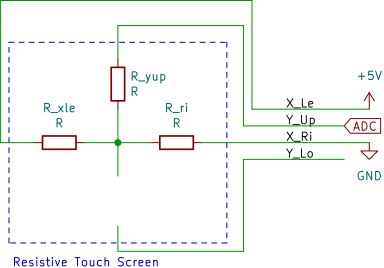
\includegraphics[width=\textwidth]{fig/xlesen.png}
        \caption{in x-Richtung}
        \label{fig:xlesen}
    \end{subfigure}
    \hfill
    \begin{subfigure}{0.49\textwidth}
        \centering
        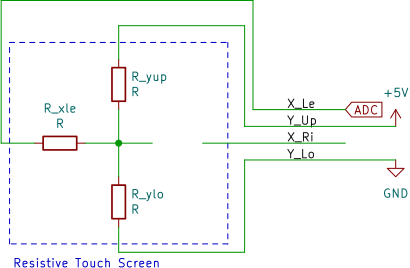
\includegraphics[width=\textwidth]{fig/ylesen.png}
        \caption{in y-Richtung}
        \label{fig:ylesen}
    \end{subfigure}
    \caption{Schaltbild für das Messen der Koordinatenpunkte}
    \label{fig:xylesen}
\end{figure}
\begin{figure}[ht!]
    \centering
    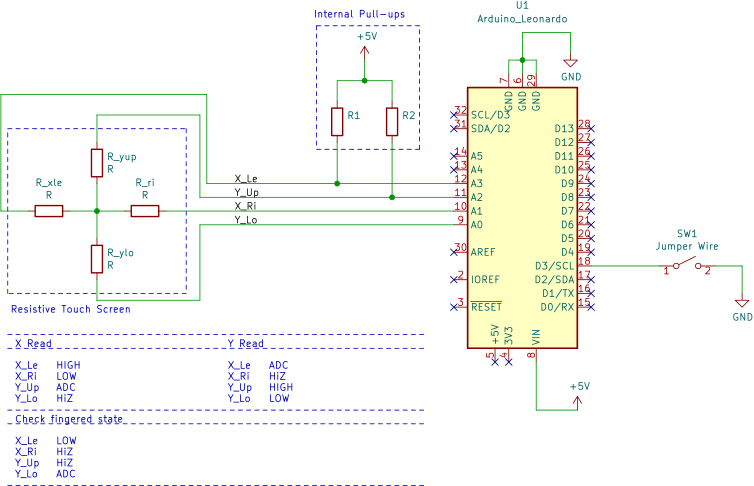
\includegraphics[width=\linewidth]{fig/schaltbild.png}
    \caption{Schaltbild des Projekts}
    \label{fig:schaltbild}
\end{figure}
Die einzelne Lösungsansätze werden in der Arduino-Umgebung umgesetzt. Der Programmablauf ist in der Abbildung \ref{fig:flowchart} auf der Seite \pageref{fig:flowchart} als Flow-Chart dargestellt.

\begin{figure}
    \centering
    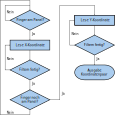
\includegraphics[scale=0.45]{fig/flow_chart.png}
    \caption{Darstellung des Programmablaufs}
    \label{fig:flowchart}
\end{figure}
\section{Umsetzung des Lösungsansatz}
\section{Filterung der Messpunkte}
    \chapter{Untersuchung der Messdaten}
Um eine Aussage über die Qualität des Touchscreen treffen zu können, werden mehrere Untersuchungen angestellt.

Bei der ersten Untersuchung wird auf die Mitte des Touchscreen gedrückt und die Position wird für eine gewisse Zeit gehalten.
Die Daten werden anschließen ausgewertet (siehe \cref{ab:genau}).

Um die erste Untersuchung zu erweitern wird nun die Mitte des Touchscreen wiederholt gedrückt.
Hier bei soll die Wiederholbarkeit eines Punktes auf dem Touchscreen untersucht werden.
Die Auswertung ist in \cref{ab:wiederholung} zu finden.

Bei der letzten Untersuchung wird die Linearität des Touchscreen untersucht.
Hierfür gibt der Hersteller eine Garantie, unter der sich die Linearität des Touchscreen befinden soll.
Den Wert der angegeben wird liegt bei \SI{1,5}{\%} (siehe \cref{ds:touch} Seite 3 des Datenblatts).

Um die Nachfolgende Untersuchungen korrekt durchführen zu können muss zu nächst der Reaktionsbereich des Touchscreens ermittelt werden.
Durch seine Bauform hat dies einen Randbereich an dem es nicht zuverlässig Werte ausgibt.
Umkehrschluss, das Programm erkennt nicht das etwas den Touchscreen betätigt.
Im Datenblatt werden Werte für den Bereich genannt in dem es zuverlässig arbeitet.
In X-Richtung hat der Touchscreen einen Arbeitsbereich von \SI{214,5}{mm} und in Y-Richtung eine Bereich von \SI{161,0}{mm}.
Diese Werte wurden durch Messungen ermittelt.

Durch Ausprobieren wurden die maximal und minimal ADC-Werte in die jeweilige Richtung ermittelt.


\begin{table}[h]
    \centering
    \caption[Empirisch ermittelter Wertebereich der ADC]{Empirisch ermittelter Wertebereich der ADC für die äußeren Grenzen des Touchscreens in jeweils horizontaler (x) und vertikaler (y) Richtung.}
    \begin{tabular}{@{}lrr@{}}
        \toprule
            &Min    &Max\\
        \midrule
        x   &68     &961\\
        y   &108    &917\\
        \bottomrule
    \end{tabular}
    \label{tab:ADC min max}
\end{table}

Mit diesen Werten lässt sich Arbeitsbereich (in ADC-Werten) des Touchscreen in jede Richtung bestimmen.
\begin{align}
    ADC_{x,len} &= 961 - 68 = 893
    \label{eq:adcxlen}\\
    ADC_{y,len} &= 917 - 108
    \label{eq:adcylen}
\end{align}
Mit diesen Werten (\cref{eq:adcxlen} und \cref{eq:adcylen}) können im Anschluss die Werte in das metrische System überführt werden und die Auflösung des Touchscreen bestimmt werden.
In x-Richtung ergibt sich eine Auflösung von \SI{0,240}{\frac{mm}{ADC}} und in y-Richtung \SI{0,199}{\frac{mm}{ADC}}.

Diese unterschiedliche Werte haben den Ursprung, dass die ADC-Werte sich in x-Richtung auf eine größere Distanz verteilen als in y-Richtung.

\section{Genauigkeit bei konstanten Koordinaten}
\label{ab:genau}
Bei dieser Untersuchung wurden zwei separate Messungen durchführen.
Im ersten Durchlauf wurden die Werte mit dem Medianfilter verarbeitet, bevor sie ausgegeben wurden.
Im zweiten Durchlauf wurden die direkten und ungefilterte Werte ausgegeben.
In den \cref{fig:filtered} und \cref{fig:unfiltered} sind die Messdaten der x- und y-Komponenten aufgetragen (siehe Seite \cref{fig:filtered}).

Die Auswertung der Messdaten ist in \cref{tab:genaufilter} und \cref{tab:genauunfilter} zu finden.
Bei der Auswertung ist zu beachten das es um zwei separate Messreihen handelt.
Daher hat auch die ungefilterte Messreihe eine Standardabweichung und Varianz von Null, im Vergleich zur gefilterten Messreihe.
Im Normalbetrieb ist der Medianfilter im Programm aktiv, daher haben die Werte der gefilterten Messreihe eine höhere Relevanz.
Die Genauigkeit des Touchscreen in beiden Messreihen ist kleiner als die Auflösung, was auf ein akkurat arbeitenden Touchscreen schließen lässt.
\begin{table}[ht!]
    \caption{Auswertung der gefilterten Messdaten }
    \begin{center}
        \begin{tabular}{ |c|c|c|c|c|c|c| }
          \hline&\multicolumn{2}{c|}{Median}& \multicolumn{2}{c|}{Standardabweichung}&\multicolumn{2}{c|}{Varianz} \\ \hline
         Einheit    &(ADC)              &mm             &(ADC)          &mm             &(ADC)      &mm\\\hline
         x-Richtung & \SI{499,0}{}      & \SI{119,861}{}&\SI{0,0}{}     &\SI{0,0}{}     &\SI{0,0}{} & \SI{0,0}{} \\  \hline
         y-Richtung & \SI{509,999}{}    & \SI{101,495}{}&\SI{0,049}{}   &\SI{0,010}{}   &\SI{0,0}{} & \SI{0,0}{} \\ \hline  
        \end{tabular}
        \label{tab:genaufilter}
    \end{center}   
    \caption{Auswertung der ungefilterten Messdaten}
    \begin{center}
        \begin{tabular}{ |c|c|c|c|c|c|c| }
          \hline&\multicolumn{2}{c|}{Median}& \multicolumn{2}{c|}{Standardabweichung}&\multicolumn{2}{c|}{Varianz} \\ \hline
          Einheit &(ADC)&mm&(ADC)&mm&(ADC)&mm\\\hline
          x-Richtung & \SI{499,0}{} & \SI{119,861}{}&\SI{0,0}{}&\SI{0,0}{}&\SI{0,0}{} & \SI{0,0}{} \\  \hline
          y-Richtung & \SI{510,0}{} & \SI{101,496}{}&\SI{0,0}{}&\SI{0,0}{}&\SI{0,0}{} & \SI{0,0}{} \\ \hline  
        \end{tabular}
        \label{tab:genauunfilter}
    \end{center}   
\end{table}


\begin{figure}[ht!]
    \centering
    \includesvg[width=\linewidth]{fig/filtered.svg}
    \caption{Darstellung der gefilterten Messreihe}
    \label{fig:filtered}
    \centering
    \includesvg[width=\linewidth]{fig/unfiltered.svg}
    \caption{Darstellung der ungefilterten Messreihe}
    \label{fig:unfiltered}
\end{figure}

\newpage

\section{Reproduzierbarkeit von Koordinaten}
\label{ab:wiederholung}
Um die Reproduzierbarkeit von Koordinaten zu untersuchen, wurde die Mitte des Touchscreen mehrmals berührt während die Messdaten aufgezeichnet wurden.
Die Auswertung der Messdaten sind in \cref{tab:wiederholung} zu sehen.
Aus den Werten kann man sagen, dass die Genauigkeit der Auflösung entspricht.
\begin{table}[ht!]
    \caption{Auswertung der Reproduzierbarkeit von Koordinaten}
    \begin{center}
        \begin{tabular}{ |c|c|c|c|c|c|c| }
          \hline  
         &\multicolumn{2}{c|}{Median}& \multicolumn{2}{c|}{Standardabweichung}&\multicolumn{2}{c|}{Varianz} \\ \hline
         Einheit    &(ADC)              &mm             &(ADC)          &mm             &(ADC)          &mm\\\hline
         x-Richtung & \SI{510,75}{}    & \SI{122,683}{}&\SI{0,894}{}   &\SI{0,215}{}   &\SI{0,8}{}     & \SI{0,192}{} \\  \hline
         y-Richtung & \SI{515,858}{}    & \SI{102,661}{}&\SI{1,159}{}   &\SI{0,231}{}   &\SI{1,3}{}     & \SI{0,259}{} \\ \hline  
        \end{tabular}
        \label{tab:wiederholung}
    \end{center}   
\end{table}


\begin{figure}[ht!]
    \centering
    \includesvg[width=\linewidth]{fig/wiederholung.svg}
    \caption{Darstellung der Reproduzierbarkeit von Koordinaten}
    \label{fig:wiederholung}
\end{figure}

\section{Linearität in x- und y-Richtung}
\label{ab:linear}
Um eine Aussage über die Linearität des Touchscreens treffen zu können, wurden in x- und y-Richtung, auf dem Touchscreen alle \SI{10}{mm} eine Markierung gesetzt (siehe \cref{fig:messlinear}).

Die jeweilige Komponenten wurde anschließend jeweils über die physikalische Strecke in einem Diagramm dargestellt (siehe \cref{fig:xlinear} und \cref{fig:ylinear}).
Die Messwerte wurden mittels einer linearen Anpassung gefittet (siehe \cref{fig:xfit} und \cref{fig:yfit}).

Das \(\chi^2\) gibt Auskunft darüber in welchem Maß Werte miteinander sich verändern.
Je kleiner dieser Wert ist desto eher stimmt die Linearität überein.
Bei der linearen Anpassung in x-Richtung wurde ein \(\chi^2\) von \(0,294\) ermittelt.
Für die Linearität in y-Richtung wurde ein \(\chi^2\) von \(5,946\) ermittelt.

Bei der Untersuchung, der Linearität in y-Richtung, gibt es bei Abstand 40 mm ein Messpunkt der von der Messpunktewolke und der dazugehörigen linearen Anpassung abweicht. Dieser Messpunkt führt zu diesem größeren \(\chi^2\) als im Vergleich zur Messreihe  in x-Richtung.

Um Abschließend eine Aussage treffen zu können, ob diese Werte im Wertebereich des Datenblatts sind (\cref{ds:touch}, \cpageref{ds:touch}), muss der Grenzwert der Chi-Quadrat-Verteilung mit den Werten der Linearen Anpassung verglichen werden.
Im Datenblatt wird eine Linearität von \SI{1,5}{\%} garantiert.
In der Wertetabelle von \cite{papula} gibt es nur Werte für \SI{1}{\%} oder \SI{2,5}{\%}.
Der gelistete Wert für zwei Freiheitsgrade und für \SI{1}{\%} liegt bei 7,88.
Sowohl das \(\chi^2\) in x-Richtung wie auch in y-Richtung ist kleiner diesem Werte.
Dies hat zur Folge, dass dieser Touchscreen eine Linearität von unter \SI{1}{\%} aufweist.
\begin{figure}
    \begin{minipage}{0.49\linewidth}
        \centering
        \includegraphics[width=\linewidth]{fig/xfit.png}
        \caption{Auswertung der Linearität in x-Richtung}
        \label{fig:xfit}
    \end{minipage}
    \begin{minipage}{0.49\linewidth}
        \centering
        \includegraphics[width=\linewidth]{fig/yfit.png}
        \caption{Auswertung der Linearität in y-Richtung}
        \label{fig:yfit}
    \end{minipage}
\end{figure} 
\begin{figure}[ht!]
    \centering
    \includegraphics[width=0.6\linewidth]{fig/messlinear.jpg}
    \caption{Messaufbau für Linearität in x- und y-Richtung}
    \label{fig:messlinear}
\end{figure}

\begin{figure}[ht!]
    \centering
    \includesvg[width=\linewidth]{fig/8_linearitaet_x.svg}
    \caption{}
    \label{fig:xlinear}
    \includesvg[width=\linewidth]{fig/8_linearitaet_y.svg}
    \caption{}
    \label{fig:ylinear}
\end{figure}

    \chapter{Fazit}
\section{Qualität der Erkenntnisse}
Der uns ausgehändigte Touchscreen weißt zum einen eine ausgeprägte Genauigkeit wie auch Linearität auf. Es entspricht den Erwartungen und arbeitet zuverlässig.
Vor allem wenn ein Punkt übe längere Zeit bedrückt wird, weißt der Touchscreen eine hohe Genauigkeit auf. 
\section{Verbesserungsvorschläge}
    \appendix
    \chapter{Anhang}
	\section{Touchscreen}
		\label{ds:touch}
		\includepdf[pages=-]{append/4_wire_standard_ds_rohs-10613.pdf}
	% \section{Messdaten}
	% 	\begin{table}[ht!]
	% 		\begin{minipage}{0.49\linewidth}
	% 			\centering
	% 			\caption{Wertetabelle der gefilterten Genauigkeit}
	% 			\DTLsetseparator{;}
	% 			\DTLloaddb{scores}{messung/genauigkeitfiltered.csv}
	% 			\begin{tabular}{|c|c|}%
	% 				\hline x (ADC)& y (ADC)% specify table head
	% 				\DTLforeach{scores}{\x=x,\y=y}
	% 				{\\\hline\x & \y}\\
	% 				\hline
	% 			\end{tabular}
	% 			\label{tab:messgenaufilter}
	% 		\end{minipage}
	% 		\begin{minipage}{0.49\linewidth}
	% 			\centering
	% 			\caption{Wertetabelle der ungefilterten Genauigkeit}
	% 			\DTLsetseparator{;}
	% 			\DTLloaddb{score}{messung/genauigkeitunfiltered.csv}
	% 			\begin{tabular}{|c|c|}%
	% 				\hline x (ADC) & y (ADC)% specify table head
	% 				\DTLforeach{score}{\x=x,\y=y}
	% 				{\\\hline\x & \y}\\
	% 				\hline
	% 			\end{tabular}
	% 			\label{tab:messgenauunfilter}
	% 		\end{minipage}
	% 	\end{table}
    \chapter{Firmware}
\definecolor{codelilas}{RGB}{170,55,241}

\definecolor{codegreen}{rgb}{0,0.6,0}
\definecolor{codegray}{rgb}{0.5,0.5,0.5}
\definecolor{codepurple}{rgb}{0.58,0,0.82}
\definecolor{backcolour}{rgb}{0.95,0.95,0.92}
\lstdefinestyle{c}{language=C++,%
    basicstyle=\footnotesize,%
    inputencoding=latin1,%
    breaklines=true,%
    stepnumber=2,% line numbering steps
    morekeywords={ones,height,width,datetime},% additional keywords to highlight
    keywordstyle=\color{blue},%
    frame=none,%
    identifierstyle=\color{black},%
    stringstyle=\color{codelilas},%
    commentstyle=\color{codegreen},%
    showstringspaces=false,%without this there will be a symbol in the places where there is a space
    numbers=left,%
    numberstyle={\tiny \color{black}},% size of the numbers
    numbersep=9pt,% this defines how far the numbers are from the text
}
\lstinputlisting[caption=Main, label=lst:main cpp, language=C++, style=c]{src/main.cpp}
\newpage
\lstinputlisting[caption=Helper Functions, label=lst:helper cpp, language=C++, style=c]{src/helper_functions.cpp}
\newpage
\lstinputlisting[caption=Defines, label=lst:defines h, language=C++, style=c]{src/defines.h}
% \newpage
% \begin{lstlisting}[language=c++]
% 	\input{src/defines.cpp}
% \end{lstlisting}
% \newpage
% \begin{lstlisting}[language=c++]
% 	\input{src/helper_functions.cpp}
% \end{lstlisting}
\end{document}